\begin{figure*}[t]
\centering
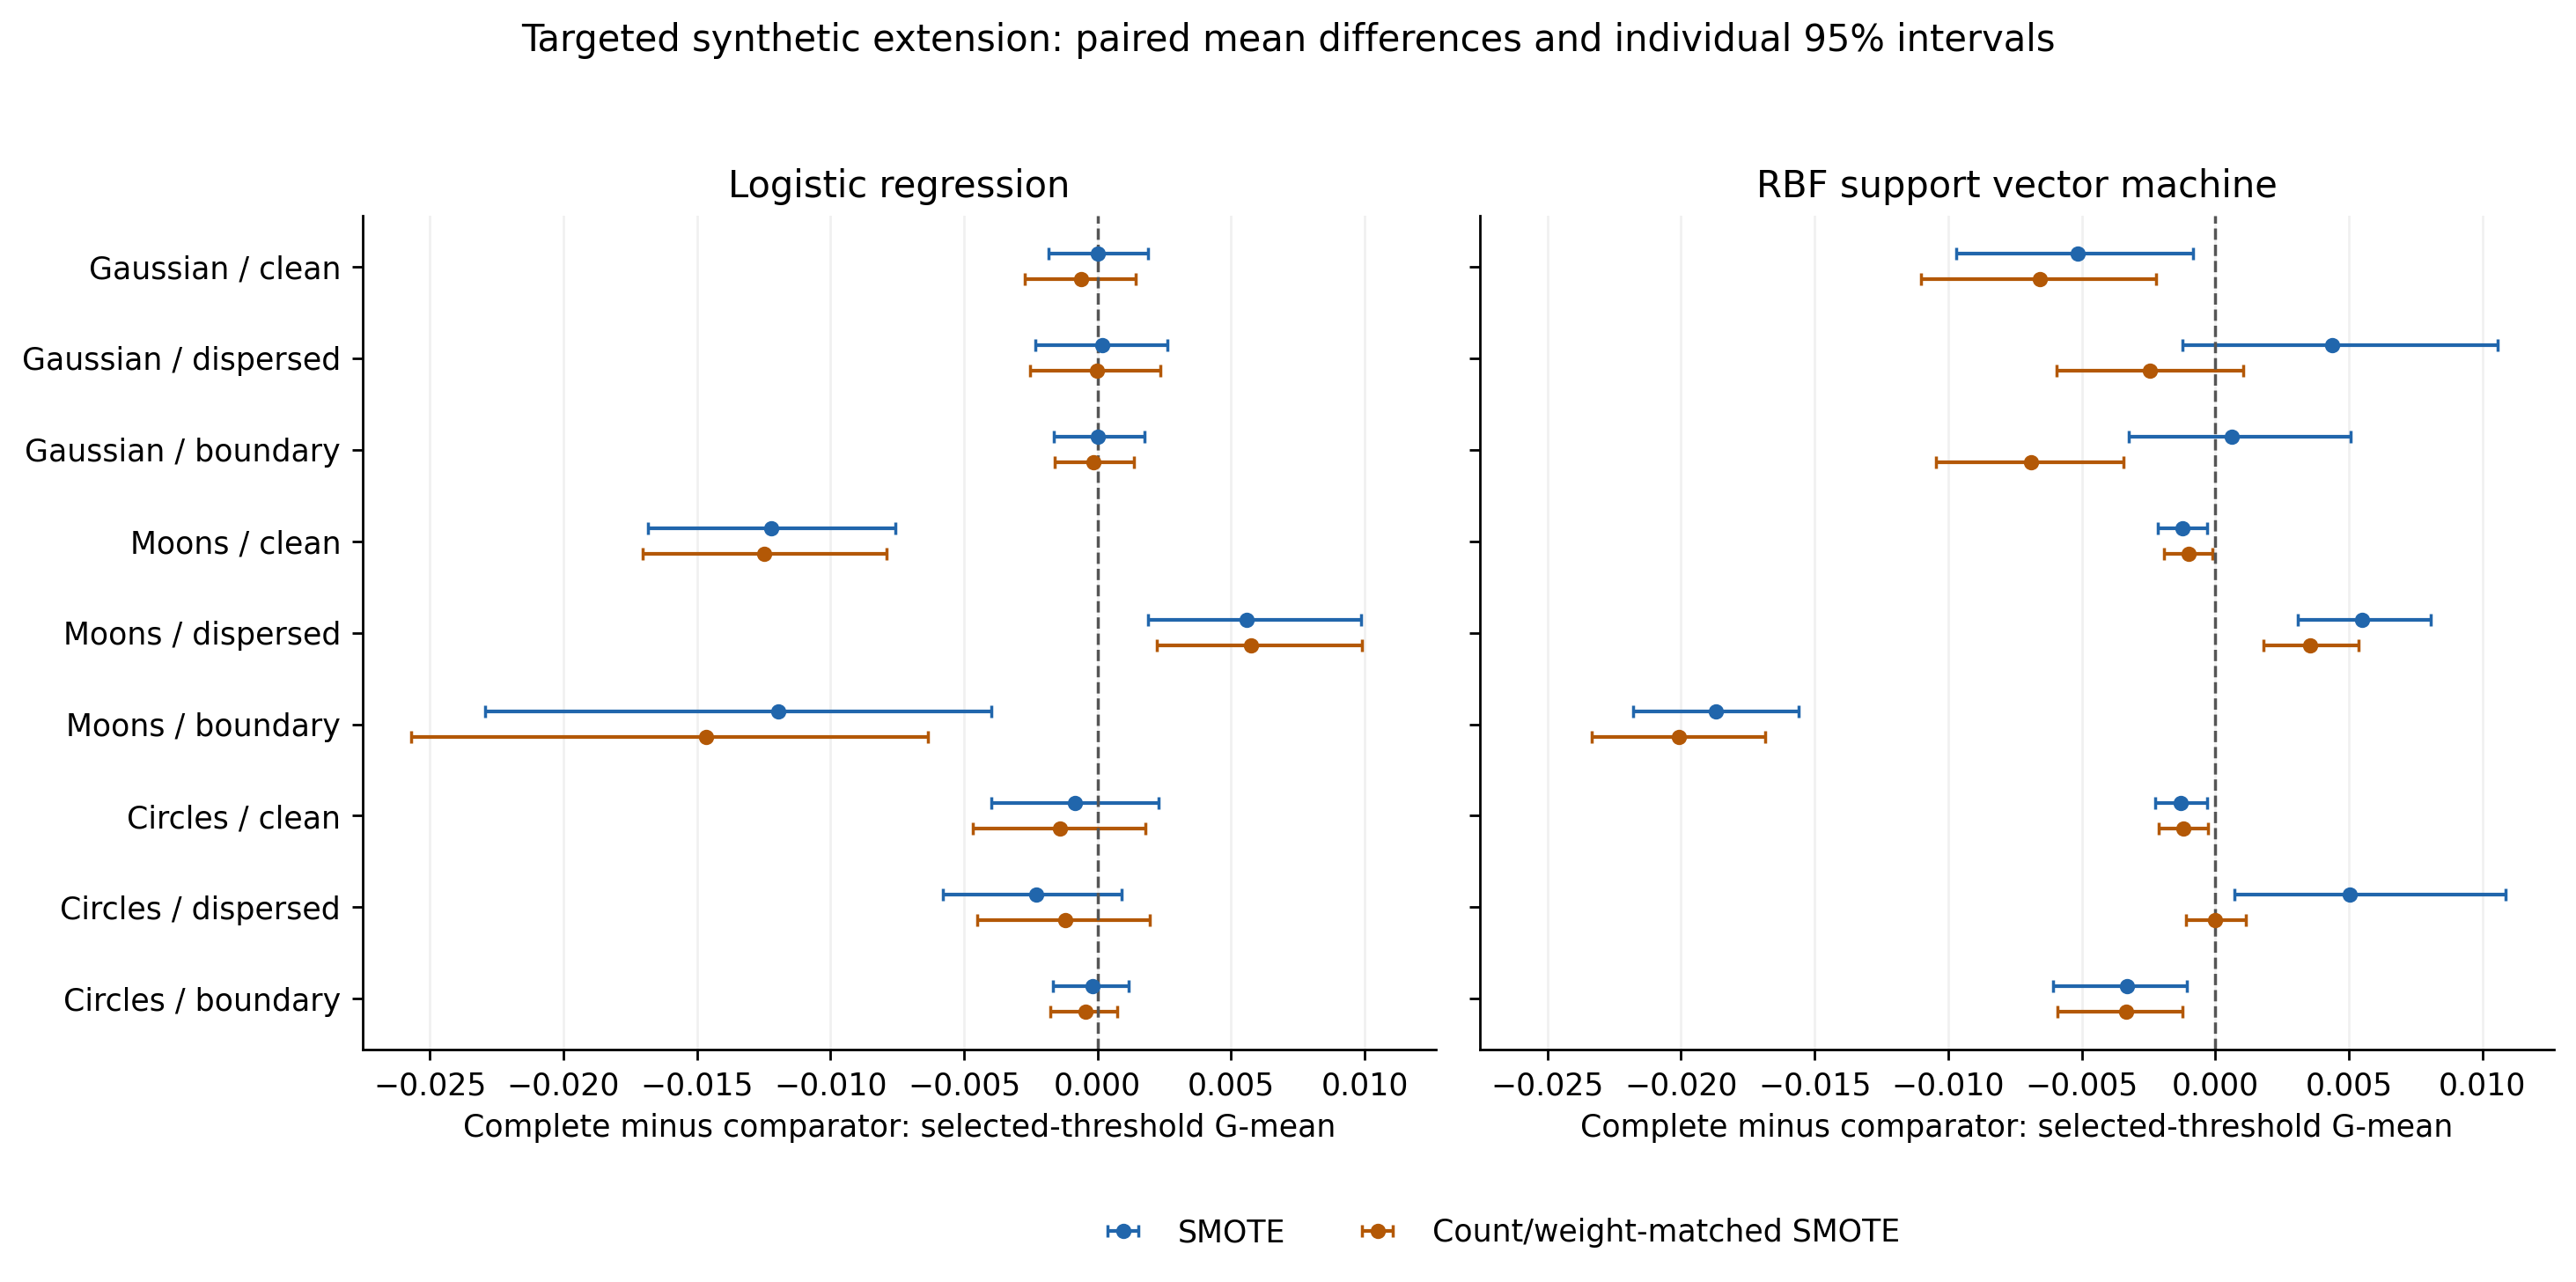
\includegraphics[width=\textwidth]{paired_gmean_intervals.png}
\caption{Paired Complete-minus-comparator G-mean after validation-based threshold selection in the targeted extension. Bars are individual 95\% paired percentile bootstrap intervals from 30 replications and 5000 resamples per setting. They are exploratory and do not provide simultaneous coverage. Matched SMOTE preserves Complete's synthetic count, original weights, and synthetic-weight multiset, with synthetic weights independently permuted over SMOTE-generated observations.}
\label{fig:targeted_paired_intervals}
\end{figure*}

Figure~\ref{fig:targeted_paired_intervals} shows the uncertainty of the setting-specific differences. Favorable and adverse outcomes remain after threshold selection, and the matched control does not reveal a consistent advantage for Complete. Supplementary Tables S1--S2 report the numerical intervals; further supplementary tables provide all baseline means, comparisons on common complete datasets, and fitting-failure counts. These comparisons retain the original evaluation protocols and do not introduce new model fits.
